% Start point: Porter model Author: Charles-Axel Dein URL: http://www.texample.net/tikz/examples/porter-model/
\documentclass{beamer}

\setbeamersize{text margin left=0mm,text margin right=0mm}

\renewcommand{\rmdefault}{bch} % change default font
\usepackage{adjustbox}
\usepackage[english]{babel}
\usepackage[utf8]{inputenc}
\usepackage{tikz} 
\usetikzlibrary{arrows,decorations.pathmorphing,backgrounds,fit,positioning,shapes.symbols,chains}

\begin{document}

\begin{frame}{}
\begin{adjustbox}{max totalsize={\textwidth}{.9\textheight},center}

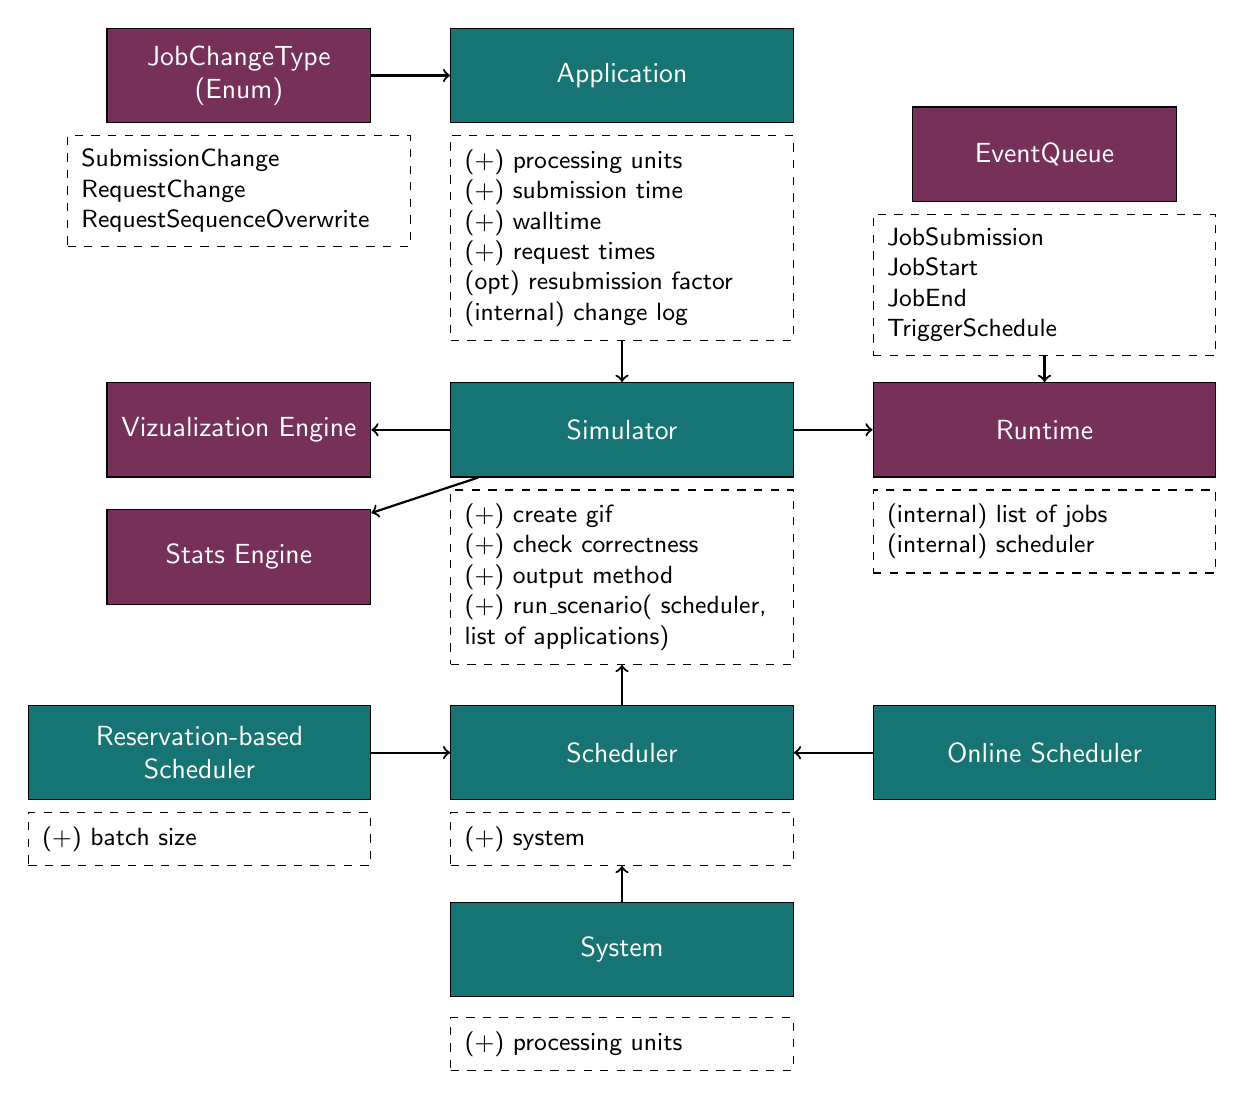
\begin{tikzpicture}
[node distance = 1cm, auto,font=\footnotesize,
% STYLES
every node/.style={node distance=3cm},
% The comment style is used to describe the methods of each class
old_comment/.style={rectangle, inner sep= 5pt, text width=4cm, node distance=0.25cm, font=\small\sffamily},
comment/.style={rectangle, draw, dashed, inner sep= 5pt, text width=4cm, node distance=0.25cm, font=\small\sffamily},
% Define styles for each type of class
api/.style={rectangle, draw, fill={rgb:red,31;green,164;blue,163}, inner sep=5pt, text width=4cm, text badly centered, minimum height=1.2cm, text=white, font=\sffamily},
extension/.style={rectangle, draw, fill={rgb:red,200;green,234;blue,253}, inner sep=5pt, text width=4cm, text badly centered, minimum height=1.2cm, text=white, font=\sffamily},
internal/.style={rectangle, draw, fill={rgb:red,96;green,39;blue,73}, inner sep=5pt, text width=4cm, text badly centered, minimum height=1.2cm, text=white, font=\sffamily}] 

% Draw classes
\node [internal] (runtime) {Runtime};
\node [internal, text width=3cm, above of=runtime, node distance=3.5cm] (eventq) {EventQueue};

\node [api, left=1cm of runtime] (simulator) {Simulator};
\node [internal, text width=3cm, left=1cm of simulator] (vizual) {Vizualization Engine};
\node [internal, text width=3cm, below=0.4cm of vizual] (stats) {Stats Engine};

\node [api, above of=simulator, node distance=4.5cm] (application) {Application};
\node [internal, text width=3cm, left=1cm of application] (jobchange) {JobChangeType (Enum)};

\node [api, below of=simulator, node distance=4.1cm] (scheduler) {Scheduler};
\node [api, left=1cm of scheduler] (batch) {Reservation-based Scheduler};
\node [api, right=1cm of scheduler] (online) {Online Scheduler};

\node [api, below of=scheduler, node distance=2.5cm] (system) {System};

%%%%%%%%%%%%%%%

% runtime
\node [comment, below=0.15 of runtime] (comment-runtime) {(internal) list of jobs\\
(internal) scheduler};

% simulator
\node [comment, below=0.15 of simulator] (comment-simulator) {(+) create gif\\
(+) check correctness\\
(+) output method \\
(+) run\_scenario( scheduler, list of applications)};

% eventq
\node [comment, below=0.15 of eventq] (eventq-comment) {JobSubmission \\
    JobStart \\
    JobEnd \\
    TriggerSchedule};

% application
\node [comment, below=0.15 of application] (comment-application) {(+) processing units\\
(+) submission time\\
(+) walltime\\
(+) request times\\
(opt) resubmission factor\\
(internal) change log};

\node [comment, below=0.15 of jobchange] {SubmissionChange \\
    RequestChange \\
    RequestSequenceOverwrite};

% scheduler
\node [comment, below=0.15cm of scheduler] (scheduler-comment) {(+) system};

\node [comment, below=0.15cm of batch] {(+) batch size};

% system
\node [comment, below=0.25 of system] {(+) processing units};


%%%%%%%%%%%%%%%%

\path[->,thick] 
(comment-application) edge (simulator)
(simulator) edge (vizual)
(simulator) edge (stats)
(simulator) edge (runtime)
(eventq-comment) edge (runtime)
(batch) edge (scheduler)
(online) edge (scheduler)
(jobchange) edge (application)
(scheduler) edge (comment-simulator)
(system) edge (scheduler-comment);

\end{tikzpicture} 

\end{adjustbox}
\end{frame}
\end{document}